% Gráfico do Capítulo 2: crescimento das classes de complexidade.
% Compile com pdflatex; o PDF gerado é incluído no capítulo (e vira PNG no site).
\documentclass[border=4pt]{standalone}
\usepackage[utf8]{inputenc}
\usepackage[T1]{fontenc}
\usepackage{pgfplots}
\pgfplotsset{compat=1.18}
\definecolor{navy}{RGB}{23,45,80}
\definecolor{laranja}{RGB}{250,110,29}
\definecolor{cinzalogo}{RGB}{107,114,126}
\begin{document}
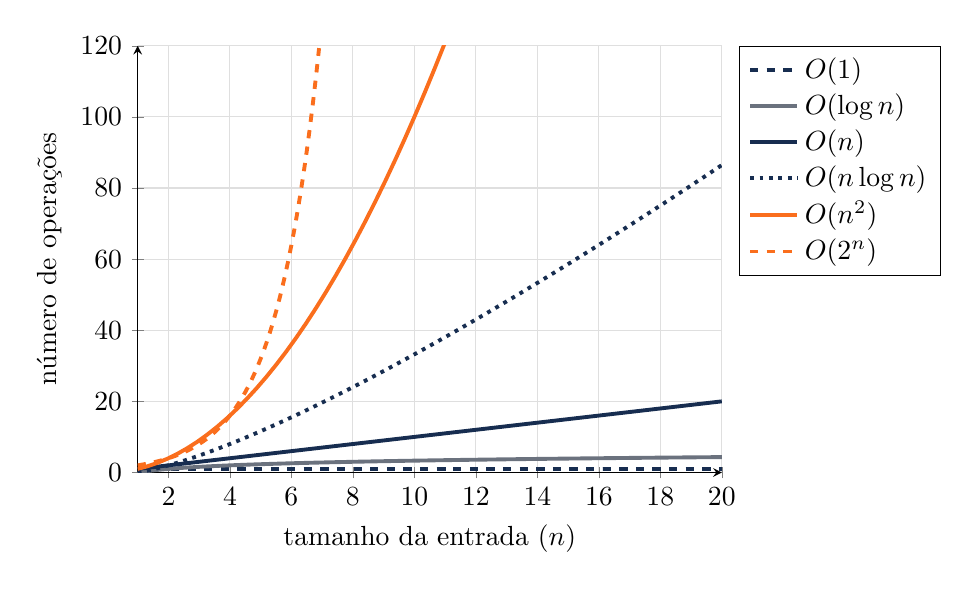
\begin{tikzpicture}
\begin{axis}[
  width=9cm, height=7cm,
  xmin=1, xmax=20, ymin=0, ymax=120,
  xlabel={tamanho da entrada ($n$)},
  ylabel={número de operações},
  legend pos=outer north east,
  legend cell align=left,
  grid=major, grid style={gray!25},
  axis lines=left,
  every axis plot/.append style={line width=1.4pt, samples=60, domain=1:20},
]
\addplot[navy, dashed] {1};                          \addlegendentry{$O(1)$}
\addplot[cinzalogo] {ln(x)/ln(2)};                   \addlegendentry{$O(\log n)$}
\addplot[navy] {x};                                  \addlegendentry{$O(n)$}
\addplot[navy, dotted] {x*ln(x)/ln(2)};              \addlegendentry{$O(n \log n)$}
\addplot[laranja] {x^2};                             \addlegendentry{$O(n^2)$}
\addplot[laranja, dashed, domain=1:6.9] {2^x};       \addlegendentry{$O(2^n)$}
\end{axis}
\end{tikzpicture}
\end{document}
